% =====================================================================
% Część II — Stan realizacji
% =====================================================================

\chapter{Geneza: etap 1 --- aplikacja bazowa PlayLink}\label{ch:real-geneza}

Projekt PlayLink Multi-Region rozwija aplikację zbudowaną w poprzednim etapie przez ten sam zespół.
Etap~1 dostarczył aplikację webową do szybkiego tworzenia i wyszukiwania sesji wspólnej gry w niszowe,
retro i mniej popularne tytuły multiplayer. Zakres obejmował interfejs użytkownika, backend z komunikacją
w czasie rzeczywistym, tworzenie, przeglądanie, dołączanie i opuszczanie sesji (pokoi), czat w pokoju,
bezhasłowe uwierzytelnianie (BIP39), kalendarz z RSVP, panel administratora oraz pełną automatyzację
wdrożenia (CI/CD). Zrealizowano wszystkie zaplanowane wymagania funkcjonalne i niefunkcjonalne, a aplikacja
działała na środowisku produkcyjnym, z naciskiem na bezpieczeństwo danych. Stos technologiczny: FastAPI,
SvelteKit, PostgreSQL, Docker Compose. Obecny etap (części II--VI kompendium) dokłada do tej bazy wymiar
wieloregionowy, powtarzalne wdrożenie, obserwowalność i serwer MCP.

\section{Zespół i podział ról w etapie 1}
\begin{table}[H]
\centering\small
\renewcommand{\arraystretch}{1.25}
\begin{tabularx}{\textwidth}{@{}p{0.27\textwidth}p{0.2\textwidth}Y@{}}
\toprule
\textbf{Osoba (nr indeksu)} & \textbf{Rola} & \textbf{Zadania} \\
\midrule
Jakub Rusek (247774) & Backend i DevOps & Architektura backendu, autoryzacja, CI/CD (GitHub Actions), strategia wdrożeń, stabilność i dostępność \\
Nikodem Nowak (251598) & Backend Developer & Logika serwerowa, API, komunikacja realtime (WebSocket), sesje i baza danych \\
Bartosz Kołaciński (251554) & Frontend Developer & Interfejs użytkownika (UI/UX), integracja frontendu z backendem \\
Mateusz Kosowski (251558) & Solution Architect & Architektura rozwiązania, spójność decyzji technicznych, koordynacja integracji \\
Jakub Rosiak (251620) & QA i dokumentacja & Scenariusze testowe, walidacja funkcji MVP, dokumentacja projektowa \\
\bottomrule
\end{tabularx}
\caption{Podział ról w zespole etapu~1.}
\end{table}
W bieżącym etapie zespół tworzą: Bartosz Kołaciński (251554), Mateusz Kosowski (251558), Nikodem Nowak
(251598), Natan Ręklewski (252952), Jakub Rosiak (251620) i Andrzej Krysiak (252945); opiekunem projektu
jest mgr inż.\ Bartłomiej Jencz.

\section{Organizacja pracy}
Pracę oparto o GitHub: Issues (planowanie i podział zadań), Projects z tablicą Kanban (Todo $\rightarrow$
Awaiting Review $\rightarrow$ Done) oraz Milestones. Obowiązywały zasady z \code{CONTRIBUTING.md}: rozwój
na gałęziach funkcyjnych, obowiązkowy przegląd Pull Requestów i konwencja komunikatów commitów. Każdy PR
musiał przejść zielony pipeline CI (lint, testy, build) przed scaleniem do \code{main}. Te zasady
obowiązują także w obecnym etapie (zasady kontrybucji: załączniki).

\section{Harmonogram etapu 1}
Etap~1 trwał 15 tygodni i został podzielony na sześć faz; testy, dokumentację i CI/CD prowadzono iteracyjnie
przez cały czas, a w harmonogramie przypisano je do tygodni, w których stanowiły główny obszar prac.

\begin{table}[H]
\centering\footnotesize
\renewcommand{\arraystretch}{1.2}
\begin{tabularx}{\textwidth}{@{}p{0.2\textwidth}p{0.13\textwidth}Y@{}}
\toprule
\textbf{Faza} & \textbf{Tygodnie} & \textbf{Zakres i kamień milowy} \\
\midrule
1. Analiza i planowanie & 1--3 & Cel i zakres, analiza platform LFG, wymagania, podział ról, backlog i Issues, wybór technologii. \emph{Zatwierdzenie założeń.} \\
2. Projektowanie & 4--5 & Architektura FastAPI--SvelteKit--PostgreSQL, REST i WebSocket, model danych, przepływ BIP39/ECDSA i sesje JWT, widoki. \emph{Gotowość do implementacji.} \\
3. Implementacja MVP & 6--8 & Szkielety backendu i frontendu, Alembic, uwierzytelnianie bezhasłowe, tworzenie, przeglądanie, dołączanie i opuszczanie pokoi, katalog gier. \emph{Działające MVP.} \\
4. Realtime i rozwój & 9--11 & Lista pokoi na żywo (WebSocket), czat pokojowy, metadane pokoi, lokalizacja lobby, filtrowanie, harmonogram i RSVP. \emph{Pełna wersja funkcjonalna.} \\
5. Bezpieczeństwo i stabilizacja & 12--13 & Rola administratora, podpisy kryptograficzne wiadomości, rate limiting, usuwanie wygasłych pokoi, poprawki UX. \emph{Zamknięcie zakresu funkcjonalnego.} \\
6. Testy i finalizacja & 14--15 & Testy backendu, frontendu i integracyjne, walidacja migracji, CI/CD, testy akceptacyjne, dokumentacja. \emph{Oddanie i wdrożenie projektu.} \\
\bottomrule
\end{tabularx}
\caption{Harmonogram etapu~1 (źródło: harmonogram realizacji projektu PlayLink).}
\end{table}

\section{Wskaźniki etapu 1}
Zdefiniowano mierzalne KPI, m.in.: co najmniej 3 przeanalizowane rozwiązania konkurencyjne, co najmniej
10 wymagań funkcjonalnych i 5 niefunkcjonalnych, co najmniej 90\% ukończonych funkcji MVP, co najmniej
3 funkcje realtime z czasem aktualizacji poniżej 1000~ms, pokrycie testami backendu co najmniej 80\%
(bramka CI), brak otwartych błędów krytycznych przed oddaniem, co najmniej 95\% zamkniętych Issues oraz
czas wdrożenia od \code{push} do live około 3~minut.

% =====================================================================
\chapter{Zrealizowane filary F1--F7}\label{ch:real-filary}

\section{Cel i zakres}
Rozdział opisuje, co zespół zbudował w projekcie \textbf{PlayLink Multi-Region}: aplikację do szukania
graczy (LFG) uruchomioną w dwóch regionach (EU i US) na Azure, razem ze sposobem wybierania regionu,
powtarzalnym wdrożeniem, eksperymentem obciążeniowym, logami z metrykami i serwerem MCP dla asystentów AI.
Opisane są tylko rzeczy faktycznie wykonane i sprawdzone. Układ odpowiada filarom F1--F7 z dokumentu wizji
(część I; źródło \code{docs/dokument-wizji.tex}). Szczegóły operacyjne (runbook, obserwowalność, konfiguracja
klientów MCP) są w części III kompendium; tu opisano, co działa, i podano wyniki.

\section{Przegląd}
\begin{table}[H]
\centering\footnotesize
\renewcommand{\arraystretch}{1.25}
\begin{tabularx}{\textwidth}{@{}l>{\raggedright\arraybackslash}p{0.2\textwidth}Y@{}}
\toprule
\textbf{Filar} & \textbf{Temat} & \textbf{Co działa} \\
\midrule
F1 & Dwa regiony z lobby & Dwa niezależne stosy (EU, US) na Azure za Cloudflare Tunnel; \code{/healthz} obu regionów zwraca wersję \code{v0.2.0-rc.2} \\
F2 & Wybór regionu & Sonda opóźnień, cookie regionu, baner Stay/Switch, automatyczny failover \\
F3 & Powtarzalne wdrożenie & \code{deploy/deploy.sh}, \code{deploy/azure-vm.sh}, wydania GHCR, aktualizacja pull-based; wydanie rc.2 wdrożone na EU i US \\
F4 & Eksperyment 1 vs 2 regiony & Runner w \code{experiments/f4/} z raportami JSON i Markdown; przebieg lokalny \\
F7 & Obserwowalność i MCP & Grafana z logami i metrykami obu regionów, serwer MCP z narzędziami do pokoi, logów i metryk \\
\bottomrule
\end{tabularx}
\caption{Zrealizowane filary projektu (stan na 18.11.2026).}
\end{table}

\section{F1: dwa regiony z działającymi lobby}
Każdy region to osobna maszyna wirtualna z własną bazą PostgreSQL, backendem FastAPI i frontendem
SvelteKit (kontenery \code{db}, \code{backend}, \code{frontend}, \code{cloudflared}). Pokoje i czat są
\emph{regionalne}, tożsamość jest wspólna (klucz z frazy BIP39 zostaje w przeglądarce). Maszyny nie mają
otwartych portów publicznych: cały ruch wchodzi tunelem Cloudflare.

\fig{architektura-regionow.png}{1.0}{Architektura dwuregionowa: gracz, Cloudflare, maszyny EU, US i ops.}

Rysunki~\ref{fig:real-eu} i~\ref{fig:real-us} pokazują tę samą aplikację w obu regionach (lokalny odpowiednik
stosu). Region EU stoi w Polsce (\code{polandcentral}), region „US'' w Danii (\code{denmarkeast}), bo Azure
for Students nie udostępnia regionów w USA; mechanizm jest identyczny.

\begin{figure}[H]\centering
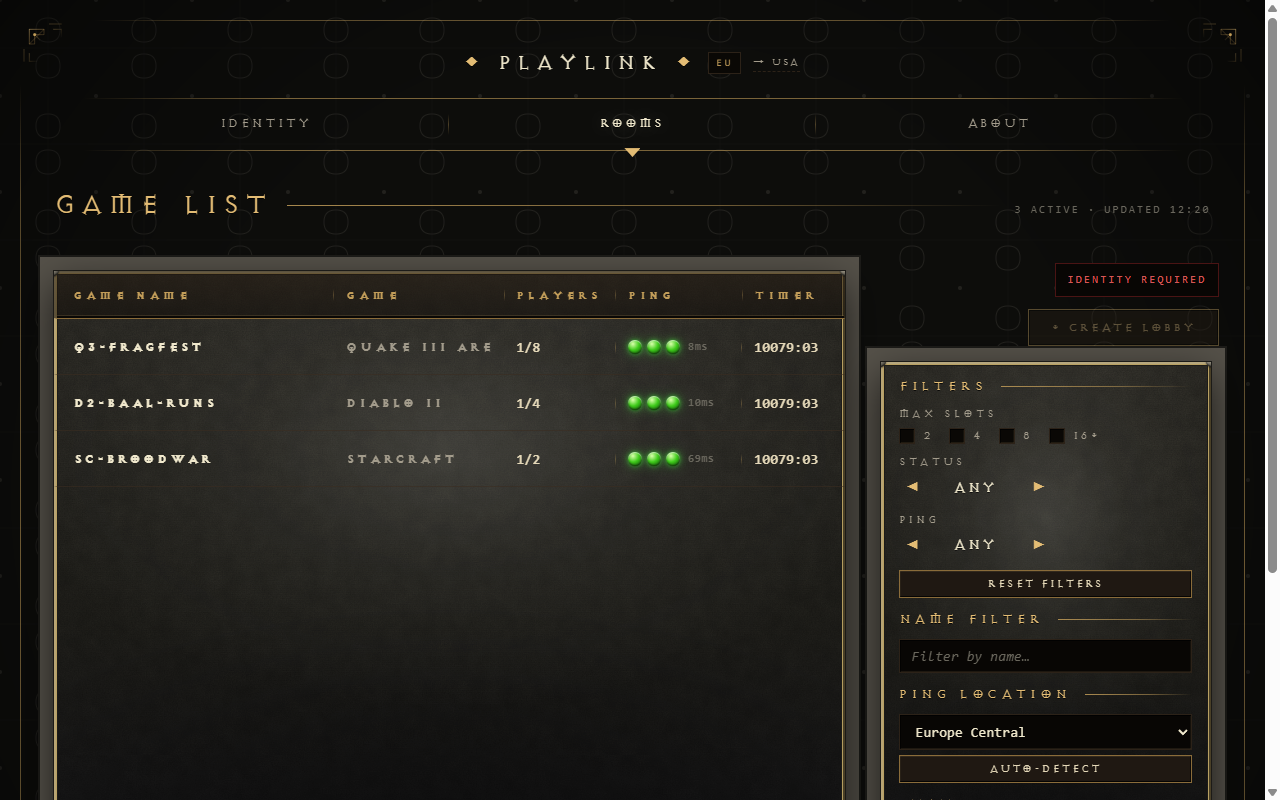
\includegraphics[width=0.8\textwidth]{02-lobby-eu.png}
\caption{Lista pokoi w regionie EU.}\label{fig:real-eu}
\end{figure}
\begin{figure}[H]\centering
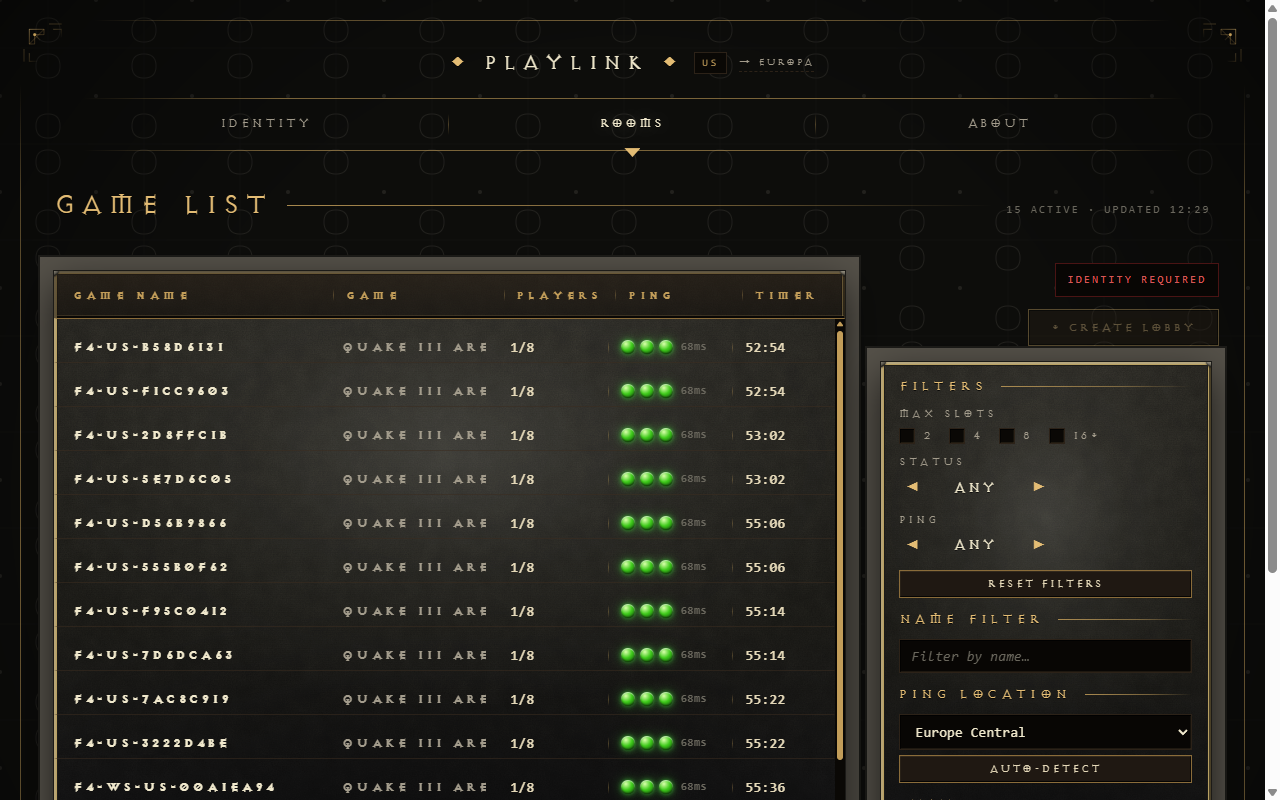
\includegraphics[width=0.8\textwidth]{03-lobby-us.png}
\caption{Lista pokoi w regionie US (pokoje utworzone przez eksperyment F4).}\label{fig:real-us}
\end{figure}

\section{F2: wybór regionu}
Przy pierwszym wejściu przeglądarka mierzy czas odpowiedzi \code{/healthz} obu regionów i otwiera lobby
w szybszym. Wybór jest zapamiętany w cookie \code{playlink.region}. Szybszy drugi region jest tylko
\emph{propozycją} (baner Stay/Switch, komponent \code{RegionProposalBanner}), a automatyczny failover
następuje wyłącznie wtedy, gdy zapisany region nie odpowiada. Ręczny przełącznik (link „→ USA'' / „→ Europa''
w layoucie) jest zawsze dostępny. Sesje są osobne dla każdego regionu (drugi login tą samą frazą mnemoniczną).
Dodatkowo czat i lista pokoi używają heartbeatu WebSocket (30~s) i automatycznie łączą się ponownie po
zerwaniu połączenia.

\fig{wybor-regionu.png}{0.75}{Przebieg wyboru regionu: sonda, zapis, propozycja i failover.}

\begin{figure}[H]\centering
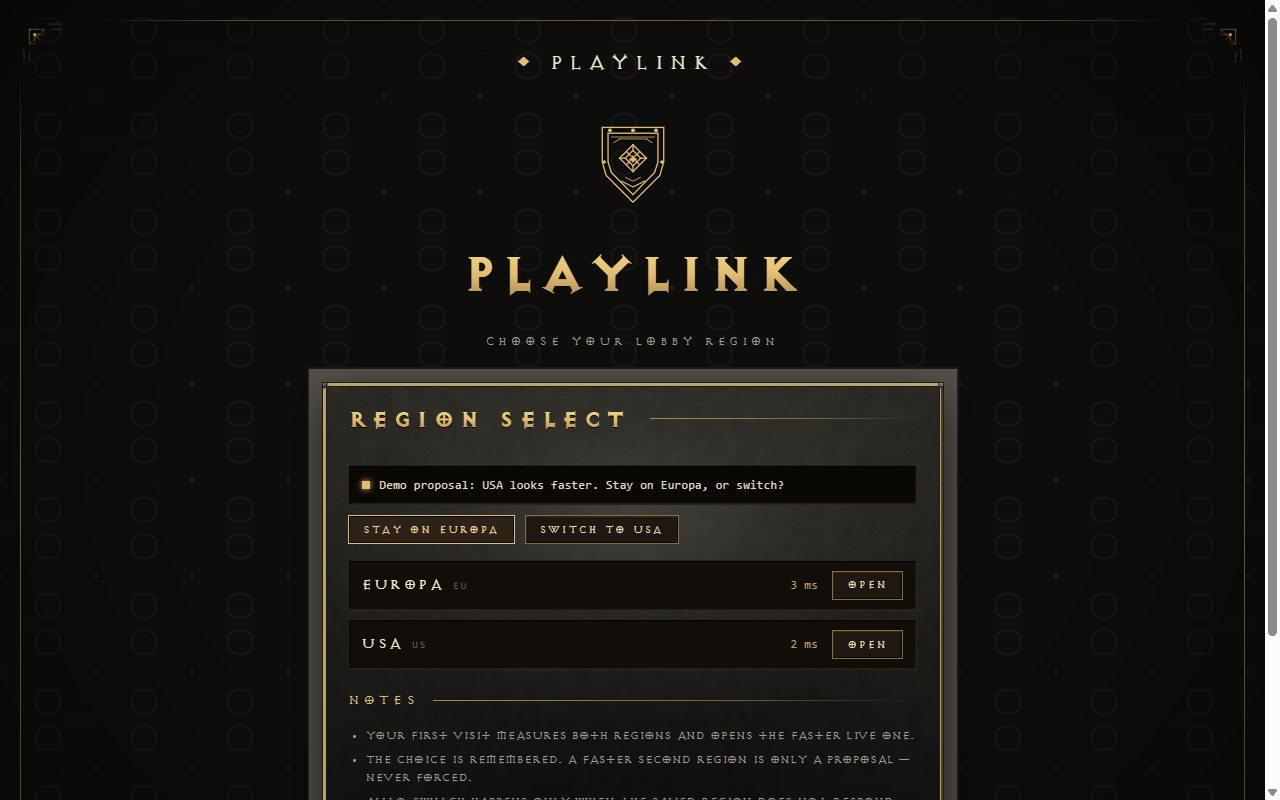
\includegraphics[width=0.85\textwidth]{01-chooser.png}
\caption{Ekran wyboru regionu z propozycją zmiany (tryb demonstracyjny \code{?propose=1}).}\label{fig:real-chooser}
\end{figure}

Reguły sprawdzone w tygodniach 5--6 (patrz dziennik etapu): pierwsze wejście trafia do szybszego żywego regionu;
gdy zapisany region żyje, a drugi jest szybszy, pojawia się baner Stay/Switch bez automatycznego przełączenia
(rys.~\ref{fig:real-chooser}); gdy zapisany region jest offline, następuje failover; odświeżenie strony nie
zmienia regionu bez akceptacji propozycji, a cookie przeżywa przeładowanie.

\section{F3: powtarzalne wdrożenie}
Jedno polecenie (\code{deploy/deploy.sh <eu|us> [tag]}) stawia region lokalnie lub na maszynie, a
\code{deploy/azure-vm.sh} tworzy całą maszynę na Azure bez otwartych portów. Wydania budują się po wypchnięciu
tagu (\code{.github/workflows/release.yml}): testy, lint, migracje, obrazy w GHCR. Maszyny same pobierają
nową wersję co 2 minuty (\code{deploy/update.sh}, timer); US czeka, aż EU zgłosi nową wersję w
\code{/healthz}, a zły release zatrzymuje się na EU i jest cofany.

Schemat wydania pull-based przedstawiono w części III, w rozdziale o wdrożeniu i wydaniach.

W praktyce: 3.11.2026 wydano \code{v0.2.0-rc.2} (kod z PR 91--102) i wdrożono je na EU, a następnie na US.
Sprawdzono wersję w \code{/healthz} obu regionów.

\section{F4: eksperyment 1 vs 2 regiony}\label{sec:real-f4}

\subsection{Cel i warianty}
Cel z dokumentu wizji (tydzień 7): zmierzyć, czy dwa regiony są szybsze niż jeden.
\begin{table}[H]
\centering\small
\begin{tabularx}{\textwidth}{@{}lll Y@{}}
\toprule
\textbf{Wariant} & \textbf{Ruch} & & \textbf{Sens} \\
\midrule
A & 100\% $\rightarrow$ EU & & punkt odniesienia „jeden region'' \\
B & naprzemiennie EU i US & & „gracz blisko swojego regionu'' \\
\bottomrule
\end{tabularx}
\end{table}

\subsection{Metodyka i scenariusze}
Runner \code{experiments/f4/run.py} porównuje oba warianty w scenariuszach: autoryzacja (nonce i podpis),
\code{list_rooms} (\code{GET /rooms}), \code{create_room} (\code{POST /rooms}), \code{join_room} i
\code{leave_room}, \code{chat_roundtrip} (WebSocket czatu: wyślij wiadomość i odbierz własny broadcast) oraz
\code{rooms_ws_update} (WebSocket \code{/ws/rooms}: czas od utworzenia pokoju do pusha listy). Dla każdego
scenariusza raport podaje: n, OK, odsetek błędów, p50, p95 i średnią (ms). Klient jest w pełni asynchroniczny
(\code{httpx.AsyncClient} i \code{asyncio.gather}); błędy, w tym 429, trafiają do raportu i nie przerywają
przebiegu. Pliki: \code{client.py} (auth, REST, WS, próbki), \code{run.py} (orkiestracja A/B),
\code{report.py} (tabele Markdown, w tym porównanie A vs B po p95 z różnicą B$-$A i pytania interpretacyjne).
Parametry \code{run.py}: \code{--variant A|B|both}, \code{--eu} (domyślnie \code{http://127.0.0.1:8000}),
\code{--us} (\code{http://127.0.0.1:8001}), \code{--users} (domyślnie 4), \code{--iterations} (domyślnie 3,
maksymalnie 3 ze względu na limit tworzenia pokoi), \code{--pace} (domyślnie 1,5~s), \code{--ws-samples}
(domyślnie 5) i \code{--out}. Wyniki trafiają do \code{experiments/f4/results/run-*.json} oraz \code{run-*.md}
(katalog w repozytorium jest obecnie pusty).

Wymagania: Python 3.11+ i dwa lokalne stosy z podniesionym limitem żądań (domyślny limit backendu to
10/minutę, za mało do testu): \code{bash scripts/local-up.sh --both --lab-limits}. Pełne polecenia
uruchomienia są w załącznikach.

\subsection{Wynik przebiegu lokalnego}
Poniżej wynik przebiegu lokalnego (4 użytkowników, 3 iteracje, dwa stosy na jednej maszynie z podniesionymi
limitami żądań).

\begin{table}[H]
\centering\footnotesize
\begin{tabular}{@{}lrrr@{}}
\toprule
\textbf{Scenariusz} & \textbf{A p95 [ms]} & \textbf{B p95 [ms]} & \textbf{Różnica B--A} \\
\midrule
GET /rooms & 24,9 & 18,6 & $-6{,}2$ \\
POST /rooms & 80,6 & 58,8 & $-21{,}8$ \\
POST /rooms/\{name\}/join & 56,8 & 49,9 & $-6{,}9$ \\
POST /rooms/\{name\}/leave & 66,0 & 49,9 & $-16{,}1$ \\
Czat WebSocket (round-trip) & 56,3 & 24,9 & $-31{,}3$ \\
Aktualizacja listy (WS) & 28,0 & 30,0 & $+2{,}0$ \\
Autoryzacja (nonce + podpis) & 135,9 & 113,9 & $-22{,}1$ \\
\midrule
\textbf{Ogółem} & \textbf{119,6} & \textbf{97,1} & \\
\bottomrule
\end{tabular}
\caption{Wynik lokalny: 91 próbek w A i 106 w B, 0\% błędów. Wariant B jest szybszy tylko dlatego, że ruch
dzieli się między dwa backendy na jednej maszynie.}
\end{table}

\subsection{Interpretacja i ograniczenia}
Hipotezy z wizji: \textbf{H1} --- dla użytkowników „USA'' wariant A jest wyraźnie gorszy niż B (p95);
\textbf{H2} --- dla użytkowników „EU'' wariant B nie pogarsza wyników względem A. Na \code{localhost} obie
hipotezy są słabo widoczne (prawie identyczny RTT), więc przebieg lokalny jest próbą generalną metody (dry-run):
potwierdza, że działa end-to-end (autoryzacja podpisem, REST, WebSocket) i daje powtarzalny raport. Rzetelny
wniosek o różnicy opóźnień wymaga uruchomienia na regionach publicznych albo generatorów obciążenia w dwóch
lokalizacjach; hipotezy H1/H2 należy uzupełnić po odczycie tabeli z takiego przebiegu. Runner działa na
dowolnych adresach, więc ten sam eksperyment można wykonać na publicznych regionach (parametry \code{--eu},
\code{--us}, np.\ \code{--users 4 --pace 2}). Scenariusze awarii regionu (zatrzymanie backendu, tunelu lub bazy)
są opisane w \code{docs/operations/runbook-regions.md}.

\section{F7: logi i metryki (Grafana)}
Każdy region ma dwa dodatkowe kontenery: Vector (wysyła logi kontenerów i metryki maszyny) i cAdvisor (metryki
każdego kontenera). Dane trafiają do osobnej maszyny \code{playlink-ops}: VictoriaLogs (logi, LogsQL),
VictoriaMetrics (metryki, PromQL) i Grafana z dashboardem „PlayLink regions''. Backend loguje JSON z
identyfikatorem żądania (\code{request_id}) i zdarzeniami biznesowymi (\code{login}, \code{room_created},
dołączanie do pokoi) oraz wystawia \code{/metrics}; błędy frontendu (serwerowe i z przeglądarki) trafiają do
tych samych logów. Grafana jest chroniona Cloudflare Access (logowanie jednorazowym kodem z e-maila), a agenty
w regionach tylko wysyłają dane, więc regiony nadal nie mają otwartych portów.

Schemat przepływu logów i metryk znajduje się w części III, w rozdziale o obserwowalności.

\begin{figure}[H]\centering
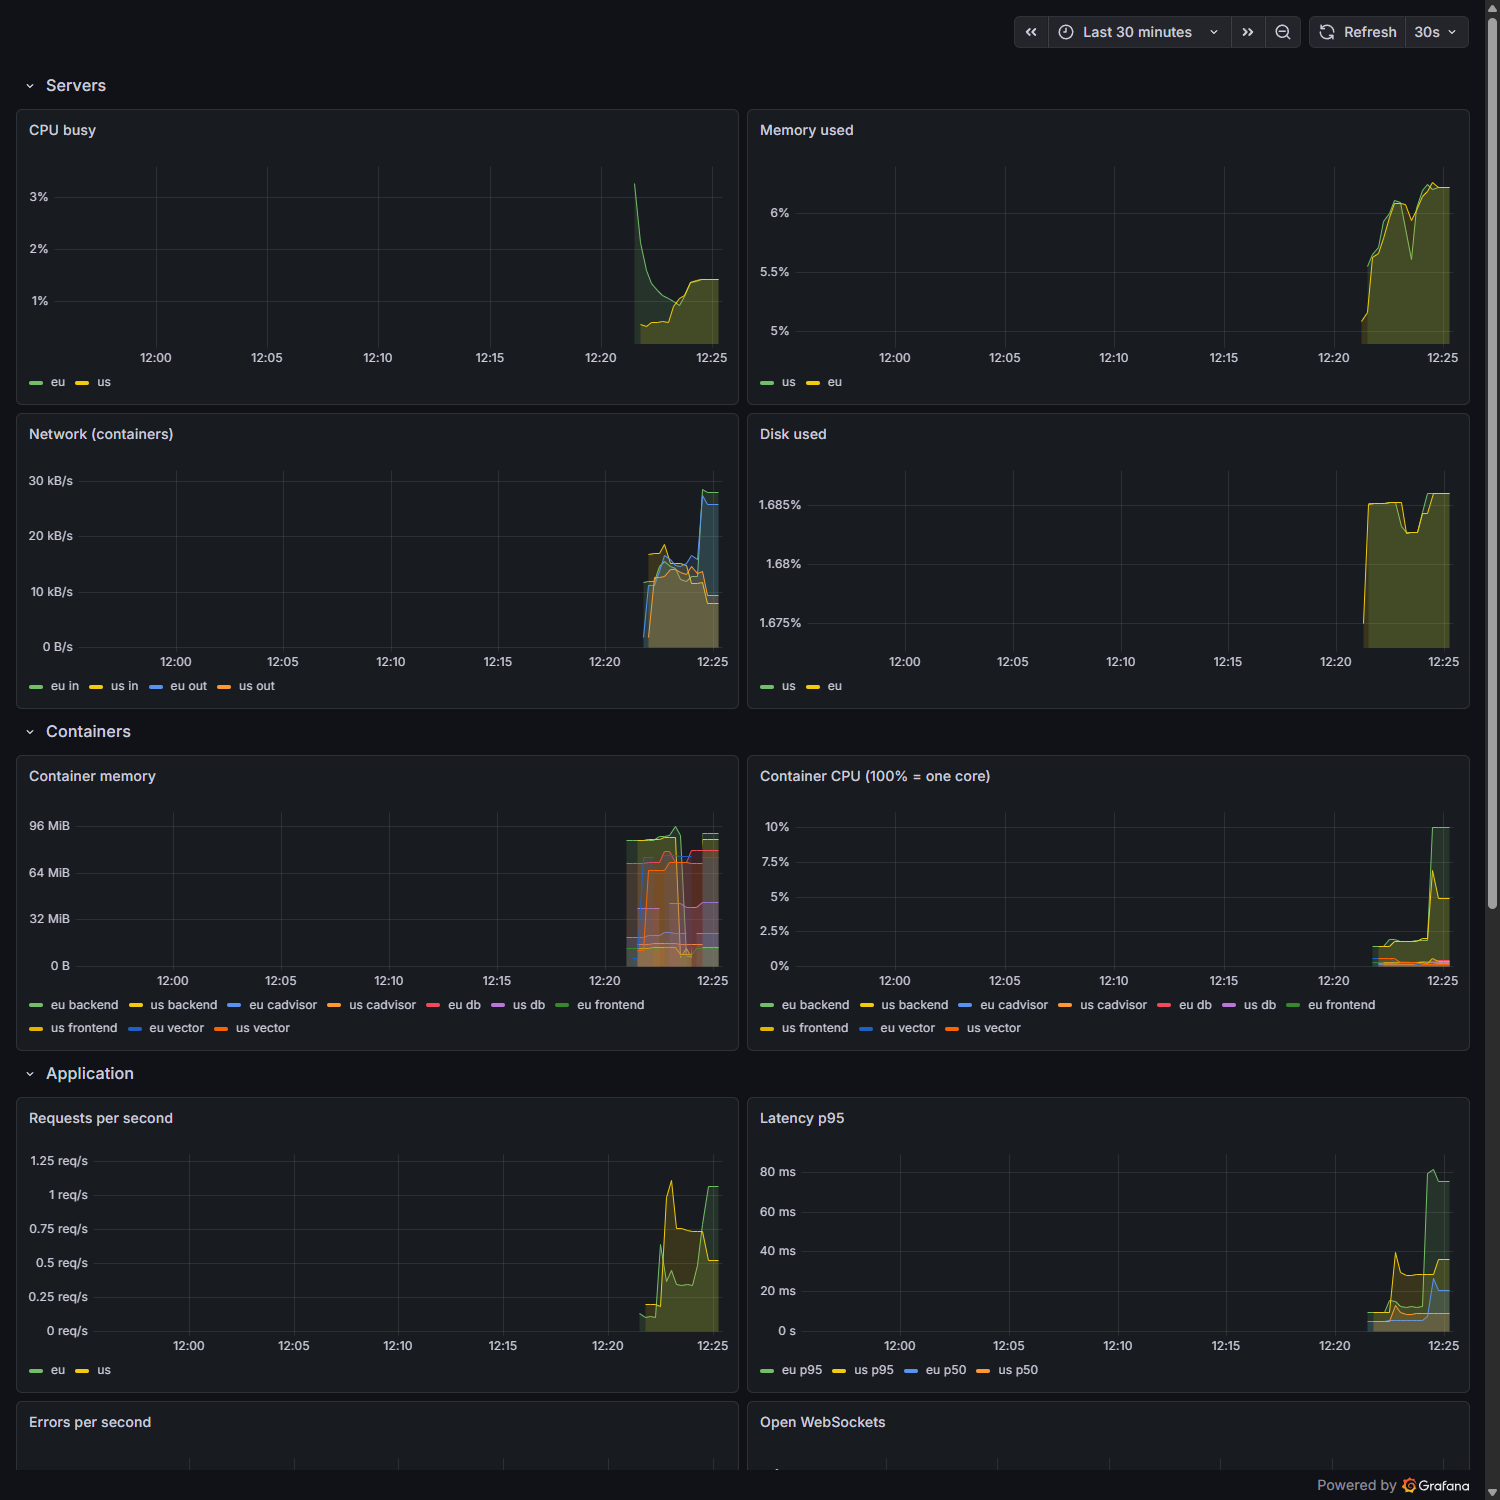
\includegraphics[width=0.95\textwidth]{04-grafana.png}
\caption{Dashboard „PlayLink regions'': zasoby maszyn i kontenerów oraz ruch i opóźnienia obu regionów
(lokalny przebieg z ruchem eksperymentu F4).}
\end{figure}

Zużycie zasobów: region z agentami potrzebuje ok.\ 250~MB RAM, stos centralny ok.\ 350~MB, więc oba mieszczą się
na maszynie z 1~GB RAM i plikiem swap.

\section{Serwer MCP}
Serwer MCP (\code{backend/mcp_server}) działa lokalnie na komputerze użytkownika, tylko do odczytu, i łączy się
z publicznym API. Daje asystentowi AI narzędzia: \code{list_games}, \code{list_rooms}, \code{get_room_details},
\code{check_platform_health}, \code{search_logs} (LogsQL) i \code{query_metrics} (PromQL). Regiony są wykrywane
dynamicznie (\code{PLAYLINK_DOMAIN}, \code{PLAYLINK_REGIONS}); błędy czasu odpowiedzi i niedostępności backendu
są zgłaszane opisowym \code{ToolError}. Sprawdzono działanie na produkcji w Azure: \code{check_platform_health}
zwrócił oba regiony jako dostępne (opóźnienie z laptopa przez Cloudflare ok.\ 127~ms dla EU i 176~ms dla US),
\code{search_logs} zwrócił świeże logi z maszyn, a \code{query_metrics} wykonał zapytanie bez błędu.
Instrukcja podłączenia dla Windows, macOS i Linuksa jest w \code{README.md} (konfiguracja klientów: część III).

Schemat połączeń serwera MCP pokazano w części III, w rozdziale o serwerze MCP.

% =====================================================================
\chapter{Wdrożenie, backlog i jakość}\label{ch:real-wdrozenie}

\section{Wdrożenie na Azure}
\begin{table}[H]
\centering\footnotesize
\begin{tabularx}{\textwidth}{@{}llYY@{}}
\toprule
\textbf{Maszyna} & \textbf{Lokalizacja} & \textbf{Rola} & \textbf{Adresy} \\
\midrule
\code{playlink-eu} & \code{polandcentral} & Region EU & \code{playlink.<domena>}, \code{playlink-eu-api.<domena>} \\
\code{playlink-us} & \code{denmarkeast} & Region „US'' & \code{playlink-us.<domena>}, \code{playlink-us-api.<domena>} \\
\code{playlink-ops} & \code{polandcentral} & Logi, metryki, Grafana & \code{playlink-grafana}, \code{-logs}, \code{-metrics} \\
\bottomrule
\end{tabularx}
\caption{Maszyny \code{Standard_B2ats_v2} (2~vCPU, 1~GB RAM), Ubuntu 24.04, bez otwartych portów.}
\end{table}
Obsługa codzienna (\code{deploy/azure.sh start|stop|status|logs}) pozwala włączać maszyny tylko na czas prób
i pokazów, żeby oszczędzać kredyt studencki. Dane przetrwają zatrzymanie, bo baza leży na dysku systemowym.

\section{Backlog zrealizowanych zadań}
\begin{table}[H]
\centering\footnotesize
\begin{tabularx}{\textwidth}{@{}p{0.2\textwidth}Yl@{}}
\toprule
\textbf{Nr} & \textbf{Zakres} & \textbf{Filar} \\
\midrule
PR 91 & Wdrożenie wieloregionowe EU/US z Cloudflare Tunnel, wydania GHCR, aktualizacja pull-based, runbook & F1, F3 \\
PR 92 & Lokalny start EU/US, propozycja Stay/Switch, eksperyment obciążeniowy & F2, F4 \\
PR 96 & Serwer MCP (tylko odczyt) & F7 \\
PR 97 & Dynamiczne wykrywanie regionów w MCP & F7 \\
PR 99, issue 94 & Logi, metryki i Grafana, błędy frontendu, narzędzia logów w MCP, maszyna ops, Cloudflare Access & F7 \\
PR 101 & Źródło LaTeX dokumentu wizji w repozytorium & dokumentacja \\
PR 102 & Instrukcja podłączenia MCP do produkcji (Windows, macOS, Linux) & dokumentacja \\
Issue 95 & Implementacja Model Context Protocol & F7 \\
Issue 103 (PR 104) & Raport, diagramy, prezentacja i aktualizacja dokumentacji & dokumentacja \\
\bottomrule
\end{tabularx}
\caption{Zrealizowane zadania; numery zweryfikowane z historią merge w repozytorium.}
\end{table}

\section{Jakość i testy}
Zmiany przechodzą CI: lint backendu i frontendu, testy (po PR 99: 159 testów backendu i 69 frontendu),
walidacja migracji w PostgreSQL, walidacja plików compose i budowanie obrazów. Przed scaleniem PR 99 wykonano
niezależny przegląd kodu, a jego uwagi naniesiono. Wydania budują się dopiero po przejściu tych samych testów.
Log wysyłki logów jest utrzymany poza bramką wydania, a endpoint błędów klienta został utwardzony (commity
PR 99).

% =====================================================================
\chapter{Dziennik etapu}\label{ch:real-dziennik}

Dziennik tygodni 1--9 prowadzono w formacie z dokumentu wizji: zaplanowane, uruchomione, wynik, wniosek.

\section{Tydzień 1: decyzje}
\begin{tabularx}{\textwidth}{@{}p{0.2\textwidth}Y@{}}
\toprule
Zaplanowane & Konto Azure for Students, rozmiar VM, budżet z alarmem \\
Uruchomione & Konto aktywne (kredyt studencki), maszyny \code{Standard_B2ats_v2} \\
Wynik & EU: \code{polandcentral}, „US'': \code{denmarkeast} (Azure for Students nie daje USA --- ten sam mechanizm) \\
Wniosek & Da się ruszać z dwoma regionami na kredytach; prawdziwy East US zostaje na później \\
\bottomrule
\end{tabularx}

\section{Tydzień 2: F1/F3, pierwszy stos EU}
\begin{tabularx}{\textwidth}{@{}p{0.2\textwidth}Y@{}}
\toprule
Zaplanowane & Przepis regionu i pierwszy stos w Europie (3 kontenery, healthcheck, baza bez internetu) \\
Uruchomione & \code{compose.yaml} i \code{deploy/deploy.sh eu} \\
Wynik & Health EU: \code{/healthz}, frontend \code{:3000}, API \code{:8000} (lokalnie) lub tunele Cloudflare (publicznie) \\
Wniosek & Jeden skrypt stawia region; nie trzeba ręcznie sklejać compose \\
\bottomrule
\end{tabularx}

\section{Tydzień 3: F1/F3, drugi region US}
\begin{tabularx}{\textwidth}{@{}p{0.2\textwidth}Y@{}}
\toprule
Zaplanowane & Ten sam przepis z plikiem US, osobna baza, te same obrazy \\
Uruchomione & \code{deploy/deploy.sh us}: projekt \code{playlink-us}, porty \code{:3001} i \code{:8001} lokalnie \\
Wynik & Oba healthchecki żywe; różnica tylko w parametrze regionu i URL-ach \\
Wniosek & Trzeci region to kolejny plik parametrów, bez zmiany architektury \\
\bottomrule
\end{tabularx}

\section{Tydzień 4: F3, CI i rollout}
\begin{tabularx}{\textwidth}{@{}p{0.2\textwidth}Y@{}}
\toprule
Zaplanowane & Ten sam commit na EU, potem US; wolumen bazy zostaje \\
Uruchomione & Release do GHCR; na VM \code{deploy/update.sh} (timer ok.\ 2 min), rollback przy złym health \\
Wynik & Tag \code{vX.Y.Z} wdraża obrazy; US czeka, aż EU zgłosi wersję \\
Wniosek & Aktualizacja pull-based wystarcza zamiast ręcznego SSH na oba hosty \\
\bottomrule
\end{tabularx}

\section{Tydzień 5: F2, routing}
\begin{tabularx}{\textwidth}{@{}p{0.2\textwidth}Y@{}}
\toprule
Zaplanowane & Sonda przed lobby, zapis regionu, \emph{propozycja} zmiany, failover tylko gdy zapisany milczy, drugi login tą samą frazą \\
Uruchomione & \code{RegionChooser}, cookie \code{playlink.region}, baner \code{RegionProposalBanner}; demo \code{?propose=1} \\
Wynik & Pierwsze wejście: szybszy żywy region; zapisany żywy i drugi szybszy: Stay/Switch (bez auto); zapisany offline: failover; sesje osobne per region \\
Wniosek & Reguła z wizji zachowana: szybszy drugi region nie przełącza sam \\
\bottomrule
\end{tabularx}

\section{Tydzień 6: F2, weryfikacja}
\begin{tabularx}{\textwidth}{@{}p{0.2\textwidth}Y@{}}
\toprule
Zaplanowane & Wejście „z EU i US'', ręczna zmiana, brak samoczynnego skoku lobby, czasy sondy, zapis po odświeżeniu \\
Uruchomione & Lokalnie \code{bash scripts/local-up.sh --both}; publicznie hosty z runbooka; link „→ USA'' / „→ Europa'' w layoucie \\
Wynik & Ręczny switch działa; odświeżenie nie zmienia regionu bez propozycji lub akceptacji; cookie przeżywa reload \\
Wniosek & Do odbioru tygodnia 6 wystarczą zrzuty choosera, banera i dwóch loginów (EU/US); F4 (obciążenie) to tydzień 7 \\
\bottomrule
\end{tabularx}

\section{Tydzień 7: F4, eksperyment 1 vs 2 regiony}
\begin{tabularx}{\textwidth}{@{}p{0.2\textwidth}Y@{}}
\toprule
Zaplanowane & Wariant A (wszyscy do EU) vs B (wybór EU/US); scenariusze: lista, pokój, join, czat WS, aktualizacja listy; tabela p50/p95 \\
Uruchomione & \code{experiments/f4/}: \code{python run.py} (AsyncClient, błędy i 429 w raporcie); start lokalny \code{scripts/local-up.sh} \\
Wynik & Pliki \code{experiments/f4/results/run-*.json} i \code{.md} (po przebiegu lokalnym lub publicznym) \\
Wniosek & Lokalnie metoda działa; sensowna różnica RTT dopiero na publicznych EU/US albo z generatorami w dwóch lokalizacjach; hipotezy H1/H2 uzupełnić po odczycie tabeli \\
\bottomrule
\end{tabularx}

\section{Tydzień 8: F7, logi, metryki i scenariusze awarii}
\begin{tabularx}{\textwidth}{@{}p{0.2\textwidth}Y@{}}
\toprule
Zaplanowane & Scenariusze awarii regionu (backend, tunel, baza) oraz wspólny podgląd logów i zużycia zasobów obu regionów \\
Uruchomione & Procedury awarii w \code{docs/operations/runbook-regions.md}; stos \code{compose.observability.yaml} na osobnej VM \code{playlink-ops}; Vector i cAdvisor w regionach (PR 99) \\
Wynik & Backend loguje JSON z \code{request_id} i zdarzeniami (\code{room_created}, \code{login}, \ldots), wystawia \code{/metrics}; błędy frontendu trafiają do tych samych logów; Grafana pokazuje oba regiony; dostęp przez Cloudflare Access (jednorazowy kod e-mail) \\
Wniosek & Cały stos obserwowalności mieści się na VM 1~GB (ok.\ 350~MB) i nie wymaga kont zewnętrznych; scenariusze awarii są opisane w runbooku \\
\bottomrule
\end{tabularx}

\section{Tydzień 9: MCP i wydanie rc.2}
\begin{tabularx}{\textwidth}{@{}p{0.2\textwidth}Y@{}}
\toprule
Zaplanowane & Inspekcja platformy przez asystentów AI oraz wydanie z całym kodem z \code{main} na oba regiony \\
Uruchomione & Serwer MCP \code{backend/mcp_server} (PR 96, 97): gry, pokoje, zdrowie regionów, dynamiczna lista regionów; narzędzia \code{search_logs} i \code{query_metrics} (PR 99); tag \code{v0.2.0-rc.2} wdrożony pull-based na EU, potem US \\
Wynik & MCP uruchomiony lokalnie łączy się z produkcją na Azure (\code{PLAYLINK_DOMAIN}, \code{PLAYLINK_REGIONS}) i zwraca zdrowie obu regionów, gry i logi; zapytania o metryki wykonują się bez błędu; instrukcja dla Linux/macOS/Windows w \code{README.md} (PR 102) \\
Wniosek & Asystent AI może odpowiadać na pytania o stan platformy bez dostępu do serwerów; hasło do logów (\code{OBS_PASSWORD}) jest jednym wspólnym sekretem, więc po oddaniu projektu należy je zmienić \\
\bottomrule
\end{tabularx}

% =====================================================================
\chapter{Wnioski}\label{ch:real-wnioski}

\begin{itemize}
  \item Dwa regiony da się stawiać i aktualizować jednym poleceniem i bez ręcznej pracy na maszynach; wystarczy
        do tego model pull-based i Cloudflare Tunnel, bez płatnych usług routingu.
  \item Maszyny nie mają otwartych portów: ruch wchodzi tunelem, a logi i metryki są wysyłane przez agentów.
  \item Lobby jest regionalne (pokoje nie są replikowane), co upraszcza system kosztem podziału społeczności graczy.
  \item Obserwowalność (logi, metryki, Grafana) mieści się na maszynach z 1~GB RAM, a serwer MCP daje asystentowi
        AI wgląd w pokoje, logi i metryki produkcji.
  \item Region „US'' stoi w Danii (\code{denmarkeast}), bo Azure for Students nie ma regionów w USA.
  \item Eksperyment F4 potwierdził poprawność metody, ale nie rozstrzyga hipotez H1/H2: wymaga przebiegu na
        publicznych regionach.
  \item Po oddaniu projektu należy zmienić wspólne hasło do logów (\code{OBS_PASSWORD}).
\end{itemize}

\section{Uruchomienie}
Procedury uruchomienia lokalnego (\code{scripts/local-up.sh}), zarządzania maszynami Azure
(\code{deploy/azure.sh}), obserwowalności (\code{deploy/observability.sh}) i podłączenia MCP są zebrane
w załącznikach oraz w części III.

% SPRZECZNOSC: lista zespołu w etapie 1 (Jakub Rusek, 247774, 5 osób) różni się od zespołu w raporcie z 18.11
% (Natan Ręklewski i Andrzej Krysiak zamiast Jakuba Ruska, 6 osób); przyjęto oba zestawy zgodnie z etapem.
% LUKA: experiments/f4/results jest puste w repozytorium (wynik lokalny podano wyłącznie z raportu); brak wyniku F4 na regionach publicznych.
